\subsection{Scheduling}\label{s:scheduling}
In der Fachliteratur wird der Begriff Scheduling mit zwar unterschiedlichen Begriffen, jedoch gleicher Bedeutung definiert. Michael Pinedo definiert Scheduling in seinem Werk \cite{mpinedo} folgendermaßen:
\begin{quote}
\textit{"`Scheduling is a decision-making process [...]. It deals with the allocation of resources to tasks over given time periods and its goal is to optimize one ore more objectives."'}
\end{quote}
So definiert er Scheduling als einen Entscheidungsprozess, der sich mit der zeitlichen Zuteilungen von Re"-ssourcen zu Aufgaben beschäftigt. Dabei ist das Ziel, ein oder mehrere Eigenschaften zu optimieren. Ferner erklärt er, dass die Ressourcen und Aufgaben in einer Organisation unterschiedliche Formen annehmen können. Ressourcen können beispielsweise Maschinen in einer Fertigungsanlage, Landebahnen auf einem Flughafen oder Verarbeitungseinheiten in einem Rechnersystem sein. Die Aufgaben wären analog Operationen in der Fertigunsanlage, Start und Landung auf dem Flughafen oder Programmausführungen im Computer. Eigenschaften der einzelnen Aufgaben sind zum Beispiel gewisse Prioritäten, frühester Startzeitpunkt oder ein Ablaufdatum. Die zu optimierende Ziele können ebenfalls viele verschiedene Formen annehmen. Das könnten die Reduzierung der gesamten Ausführungszeit einer Aufgabe sein oder die Minimierung der Anzahl von Aufgaben, die nach ihrer Fälligkeit abgeschlossen wurden.\\

Eine andere Definition ist von Alessandro Agnetis aus seinem Buch \cite{aagnetis}:
\begin{quote}
\textit{"`[...] by scheduling we mean all actions that have to be done in order to determine when each activity of a set is to start and to complete."'}
\end{quote}
So umfasst seiner Ansicht nach Scheduling diejenigen Tätigkeiten, die zur Bestimmung der Start- und Endzeit einer Aktivität aus einem Set getätigt werden müssen. Den Begriff Job spezifiziert er als Aktivität aus einem Set. So ist jeder Job im Wettkampf mit den anderen um die Nutzung von Zeit und Ressourcen. Als Ressourcen charakterisiert der Autor alles, was zur erfolgreichen Ausführung der Jobs erforderlich ist. Wie M. Pinedo benennt er Scheduling ebenso als einen Prozess, der sich mit der Zuteilung von Ressourcen zu Jobs beschäftigt. Seiner Meinung nach ist ein \textit{Schedule} (Plan) somit durch eine Menge von Startzeiten und zugeteilten Ressourcen bestimmt, der einige vordefinierte Anforderungen erfüllt.\\
Ein Problem, in welchem bei gegebenen Eingabedaten ein Plan gefunden werden muss, wird \textit{Scheduling-Problem} genannt (siehe \ref{s:probleme}). Ein \textit{feasible Schedule} (ausführbar) ist ein Plan, der alle Anforderungen des gegebenen Scheduling-Problems erfüllt \cite{aagnetis}.\\

Im Kontext des \textit{Prozess-Scheduling} erklärt Avi Silberschatz in \cite{asilberschatz}, dass dieses dafür verantwortlich ist, dass die Prozesse aus den Warteschlangen ausgeführt werden können. Dazu erteilt der Scheduler den Prozessen eine gewisse Zeit lang die CPU, in der sie diese Ressource benutzen können. Weitere Aufgaben des Prozess-Scheduling sind in Kapitel \ref{s:schedInformatik} erläutert.\\

Zusammenfassend kann also festgestellt werden, dass ein Scheduler Ressourcen und Aufgaben verwaltet. Dazu wird ein optimaler Plan erstellt, der sicherstellen soll, dass alle Aufgaben mit ihren Eigenschaften (Startzeit, Ablaufdatum, Priorität) und den benötigten Ressourcen erfolgreich ausgeführt werden. Oftmals ist es nicht einfach, einen optimalen Plan für die gegebenen Schedule-Anforderungen zu finden. Kriterien, welche durch den Scheduler optimiert werden sollen, sind in Abschnitt TODO vorgestellt.\\
\cite{mpinedo} und \cite{aagnetis} zeigen ein Beispiel, in dem die Rolle des Scheduling in einer realen Umgebung illustriert wird:
\\
\begin{description}
\item[Gate-Zuweisung am Flughafen]
An einem Airline-Terminal eines größeren Flughafens gibt es dutzende Gates und hunderte von Flugzeugen, die täglich starten und landen. Sowohl die Gates als auch die Flugzeuge sind nicht identisch. Manche Gates haben räumlich viel Platz, sodass hier auch größere Flugzeuge angekoppelt werden können. Andere sind so gelegen, dass es schwierig ist die Flugzeuge ohne Unterstützung anzukoppeln. Obwohl die Flugzeuge nach einem gewissen Plan ankommen und wieder abheben, gibt es doch zufällige Änderungen, die vom Wetter oder anderen nicht vorhersehbaren Ereignissen beeinflusst werden. Während ein Flugzeug an einem Gate steht, müssen die Passagiere die Maschine verlassen. Diese muss getankt, gereinigt und beladen werden und anschließend die Passagiere des nächsten Fluges einsteigen. Die Abflugzeit ist hier das Ablaufdatum, da bis zu diesem Zeitpunkt alle Aufgaben abgeschlossen sein müssen. Wenn jedoch absehbar ist, dass das Flugzeug nicht am Zielflughafen landen kann, wird es auch nicht abheben. Aus Vorschriftsgründen bleiben die Passagiere dann im Terminal anstatt im Flugzeug. Das Flugzeug würde für eine erweiterte Zeit am Gate stehen bleiben und blockiert es somit für andere.\\
Der Scheduler muss die Flugzeuge so den Gates zuweisen, dass dies physisch möglich ist. Dies impliziert, dass die Flugzeuge an die Gates passen und diese zur geplanten Ankunftszeit auch zur Verfügung stehen. Anforderungen wie die zeitliche Reduktion eines Arbeitsvorgangs für das Airline Personal oder die Reduzierung von Verspätungen müssen dabei optimiert werden.\\
In diesem Beispiel sind die Gates die Ressourcen und die Wartung der Flugzeuge die Aufgaben. 

%\item[Halbleiter Herstellung]
%Halbleiter werden in hoch spezialisierten Fabriken hergestellt. Meistens besteht die Herstellung aus vier Phasen: Wafer-Herstellung, Wafer-Untersuchung, Montage und finaler Test, wobei die Herstellung die komplexeste Phase ist. Die Wafer werden aus Metall- und Siliziumschichten hergestellt und jede Schicht muss einer Anzahl an Arbeitsgängen unterliegen. Manche Maschinen müssen extra für bestimmte Aufgaben vorbereitet werden. Die Anzahl an Bestellungen im Produktionsprozess liegt oft im Bereich mehrerer hundert Stück und jede Bestellung hat ihr eigenes Release- und bestätigtes Lieferdatum. Die Bestellungen werden in Jobs umgewandelt und mit Ablaufdaten verknüpft. Die Ausführung dieser Jobs kann zeitweise verspätet sein, wenn spezielle Maschinen belegt sind oder Jobs mit höherer Priorität den Aktuellen verdrängen. Unvorhersehbare Ereignisse, wie Maschinenausfälle oder eine länger als erwartete Herstellung, müssen ebenso berücksichtigt werden, da sie einen großen Einfluss auf den Schedule haben.\\
%Die Aufgabe des Schedulers umfasst die Einhaltung der maximalen Anzahl an Lieferterminen bei zeitgleicher Optimierung des Durchsatzes. Letzeres Ziel ist erfüllt, wenn die Geräteauslastung, unter anderem die der Engpassmaschinen maximiert ist. Zusätzlich müssen Ruhe- und Setupzeiten minimiert werden.
\end{description}
\begin{figure}[h]
	\centering
	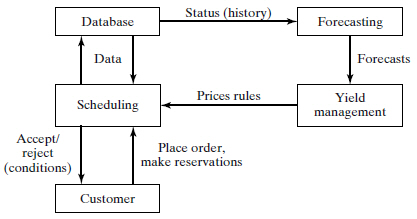
\includegraphics[width=0.45\textwidth]{pictures/info_flow_service_system}
	\caption{Informationsfluss Service-System }
	\label{f:info_flow}
\end{figure}

Diagramm \ref{f:info_flow} unterstreicht die Aussage, dass Scheduling-Systeme viele Abhängig"-keiten zu anderen Infrastrukturen besitzen können bzw. müssen. Das Diagramm zeigt den Informationsfluss in einer Service-Organisation, beispielsweise eines Autoverleihs. Dabei wird das Scheduling von Einflussgrößen wie den Kunden, der Datenbank oder auch Vorhersage-Modulen geprägt. So gehören neben den Punkten aus den oben genannten Definitionen noch folgende Aufgaben zum Scheduling:
\begin{description}
\item[planning:] Planung der Aufgaben für die einzelnen Ressourcen
\item[dispatch:] dynamische Zuteilung einer Ressource zu einer Instanz (Job)
\item[processing:] Ausführung der Instanz
\item[control:] begleitende Auftragssteuerung
\item[monitoring:] Beobachtung des Zustandes
\item[feedback:] Rückmeldung von Ergebnissen und Abschlüssen aller verketteten Teilprozesse einer Instanz
\end{description}



Zusammenfassend ergeben die Definitionen aus \cite{mpinedo} und \cite{aagnetis} einen Prozess, der die Planung und Zuteilungen von Ressourcen zu Aufgaben sowie deren Ausführung und Beobachtung beschreibt. Dazu kommt die Einbeziehung sowie Auflösung von Abhängig"-keiten zu anderen Systemen, die Start- und Endzeit einer jeden Aufgabe beeinflussen.


	